% Software Development for Mobile Devices
\documentclass[11pt,english,numbers=endperiod,parskip=half]{scrartcl}

\usepackage{color}
\usepackage{graphicx}
\usepackage{minted}
\usepackage{fancyhdr}
\usepackage{pdflscape}

\pagestyle{fancy}

\rhead{Daniel Parker - 971328X}
\lhead{COS30017 - Software Development for Mobile Devices}

\title{Assignment 06}
\subtitle{COS30017 - Software Development for Mobile Devices}
\author{Daniel Parker 971328X}

\date{\today}

\begin{document}
\maketitle
\thispagestyle{empty}

\section{Task 1 - Activities and Fragments}
The difference between activities and fragments lies primarily in their lifecycle
and where they exist in the context of an app. Firstly, Fragment is a subclass
of Activity and therefore inherits all of the Activity's primary functionality.
The difference is that an Activity can contain many fragments, and the fragments
will provide their UI to the containing Activity. This pattern also allows for
reusability of UI components in different activities.

The FragmentManager is a central class to managing fragments across an app. It
allows for searching for fragments, managing the fragments on the back stack, and
creating new FragmentTransactions. FragmentTransactions are an API for controlling
the behaviour of Fragments in an app, and what fragments are visible and also that
any changes get committed to the backstack to allow for proper back-button navigation
by the user.

\section{Task 2 - Simple Custom List}
% Source code needs landscape

\subsection{Screenshot}
\setlength\fboxsep{0pt}
\setlength\fboxrule{0.5pt}

\begin{figure}[H]
\centering{
	\fbox{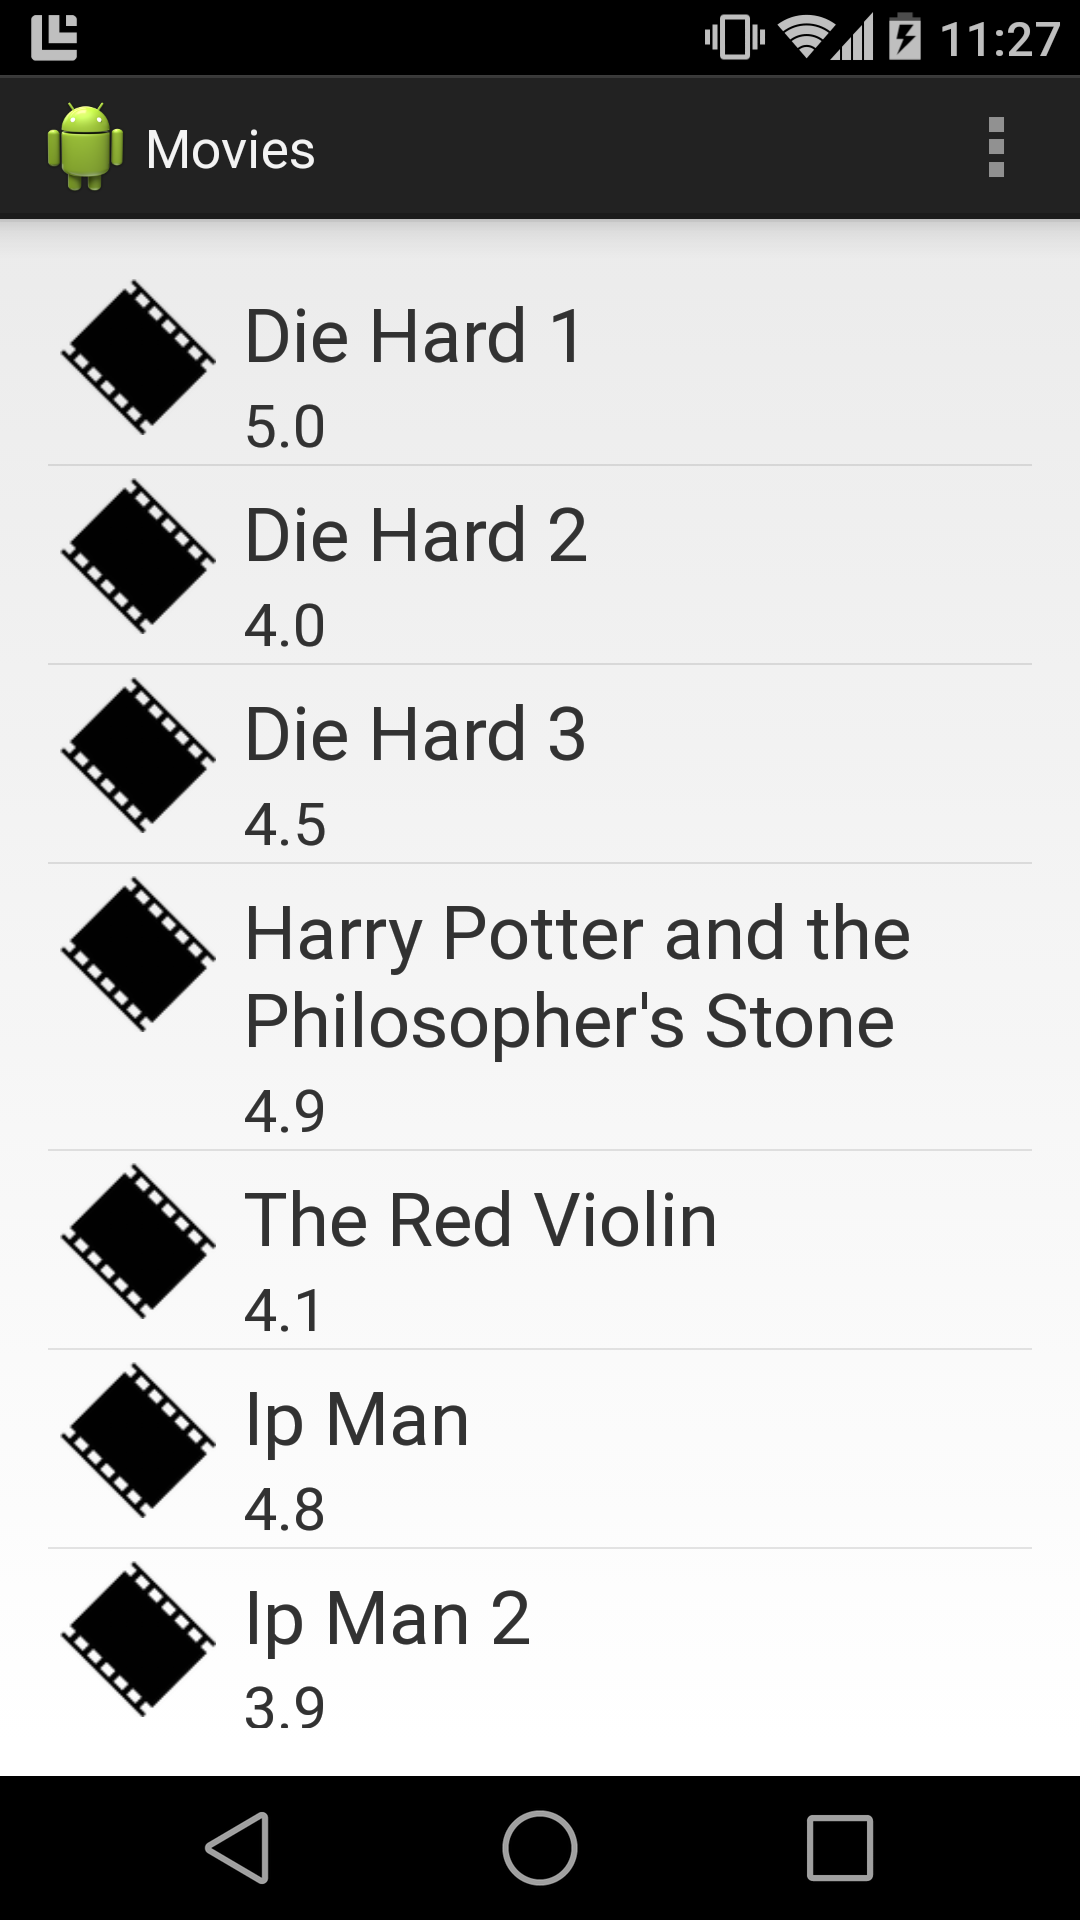
\includegraphics[width=5cm]{images/movies.png}}
}\\
\end{figure}

\begin{landscape}
\subsection{Source Code}
\subsubsection{Movie Model}
\inputminted{java}{../../Apps/Movies/app/src/main/java/au/net/danielparker/movies/Movie.java}

\subsubsection{MovieList Activity}
\inputminted{java}{../../Apps/Movies/app/src/main/java/au/net/danielparker/movies/MovieList.java}

\subsubsection{MovieListAdapter}
\inputminted{java}{../../Apps/Movies/app/src/main/java/au/net/danielparker/movies/MovieListAdapter.java}

\subsubsection{activity\_movie\_list.xml}
\inputminted{xml}{../../Apps/Movies/app/src/main/res/layout/activity_movie_list.xml}

\subsubsection{movie\_layout.xml}
\inputminted{xml}{../../Apps/Movies/app/src/main/res/layout/activity_movie_list.xml}

\end{landscape}


\section{Task 3 - Action Bar Design Pattern}
The action bar design pattern has become a very prominent visual design pattern
and is preferred to the older pattern of puttings everything on a landing dashboard.
The reasons for it's success and recommended use, are that it provides a dedicated
space for the app logo and branding, as well as the user's current location in
the app. It makes the important contextual actions for an Activity prominent,
and it provides consistent navigation when switching between apps. It also works
nicely across multiple device screen sizes and orientations.

\section{Task 4 - Add a Custom Geo Location}
The Custom Geo Location app uses the devices internal storage to allow the user
to add custom locations to get suntimes for. The modes that are used are
\textit{MODE\_PRIVATE} and \textit{MODE\_APPEND}.
\subsection{Screenshots}
\setlength\fboxsep{0pt}
\setlength\fboxrule{0.5pt}

\begin{figure}[H]
\centering{
	\fbox{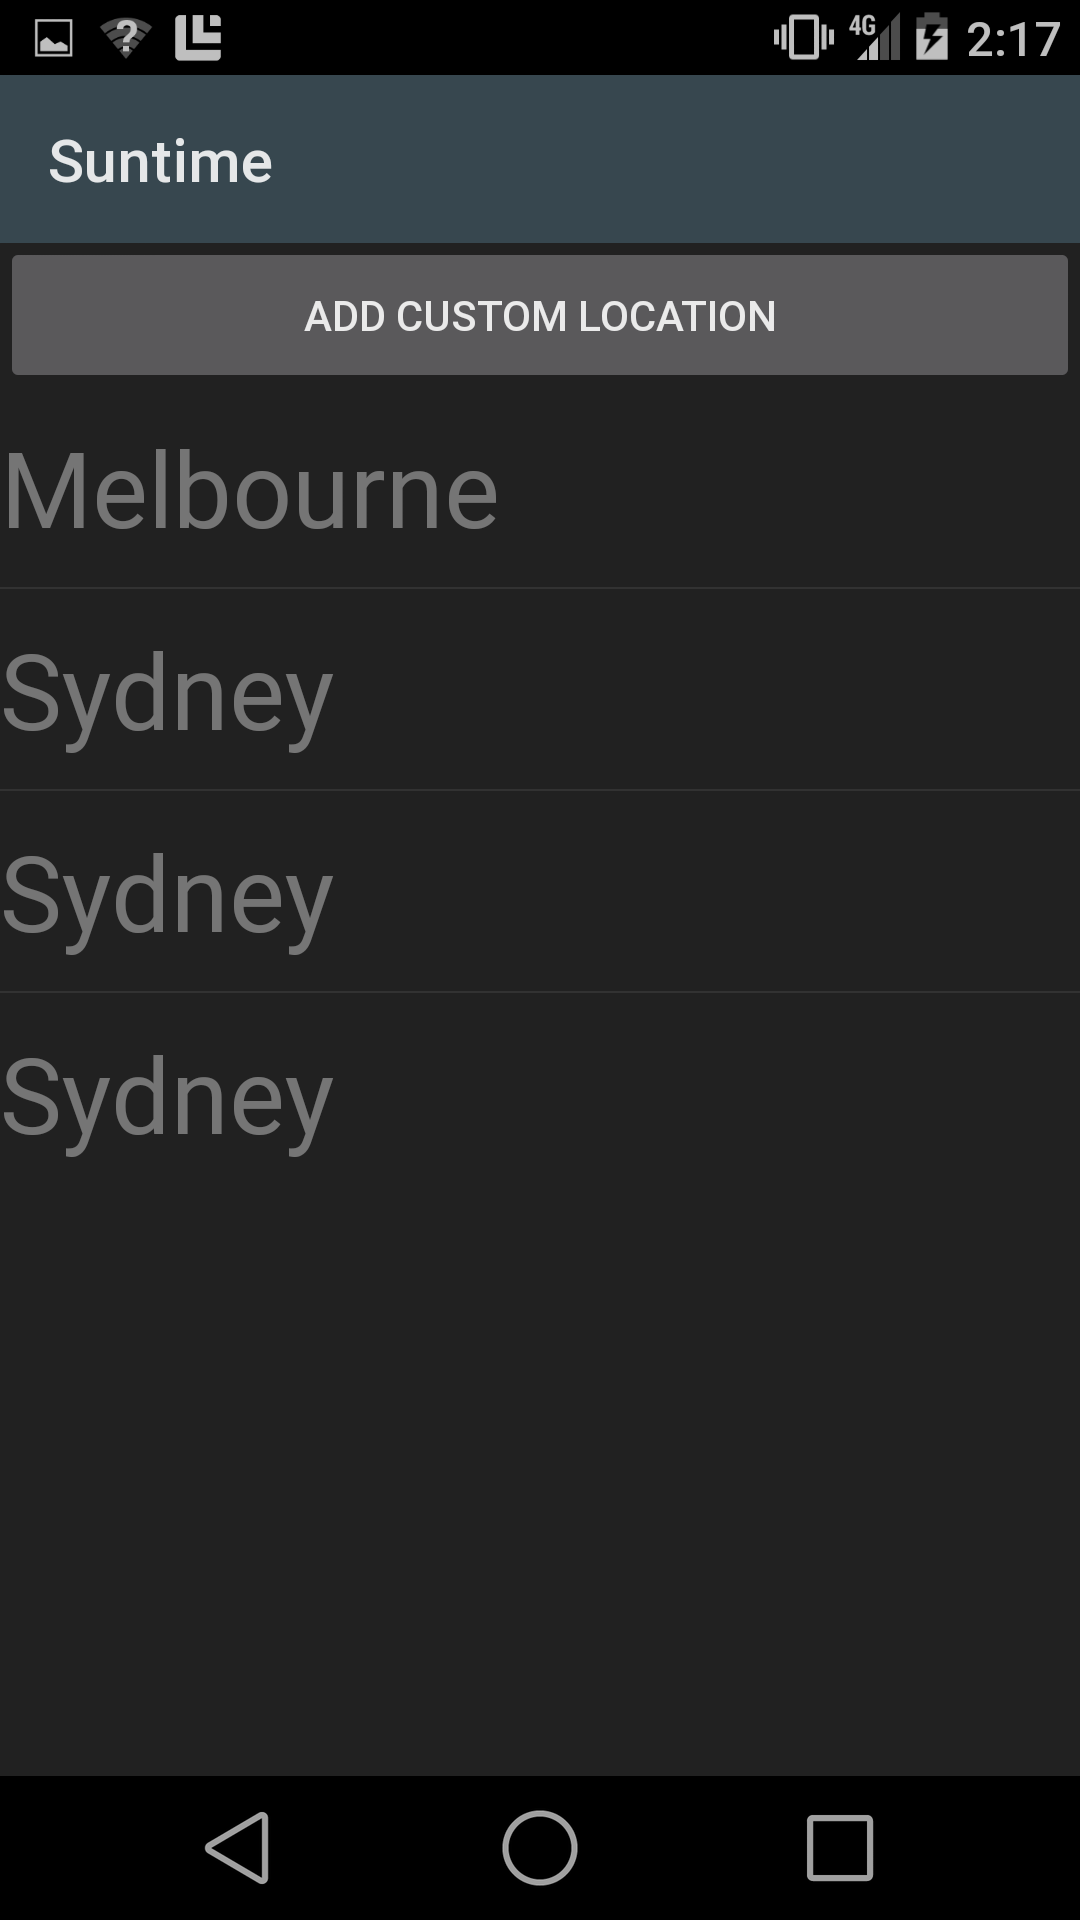
\includegraphics[width=5cm]{images/list.png}}
}\\
\end{figure}

\begin{figure}[H]
\centering{
	\fbox{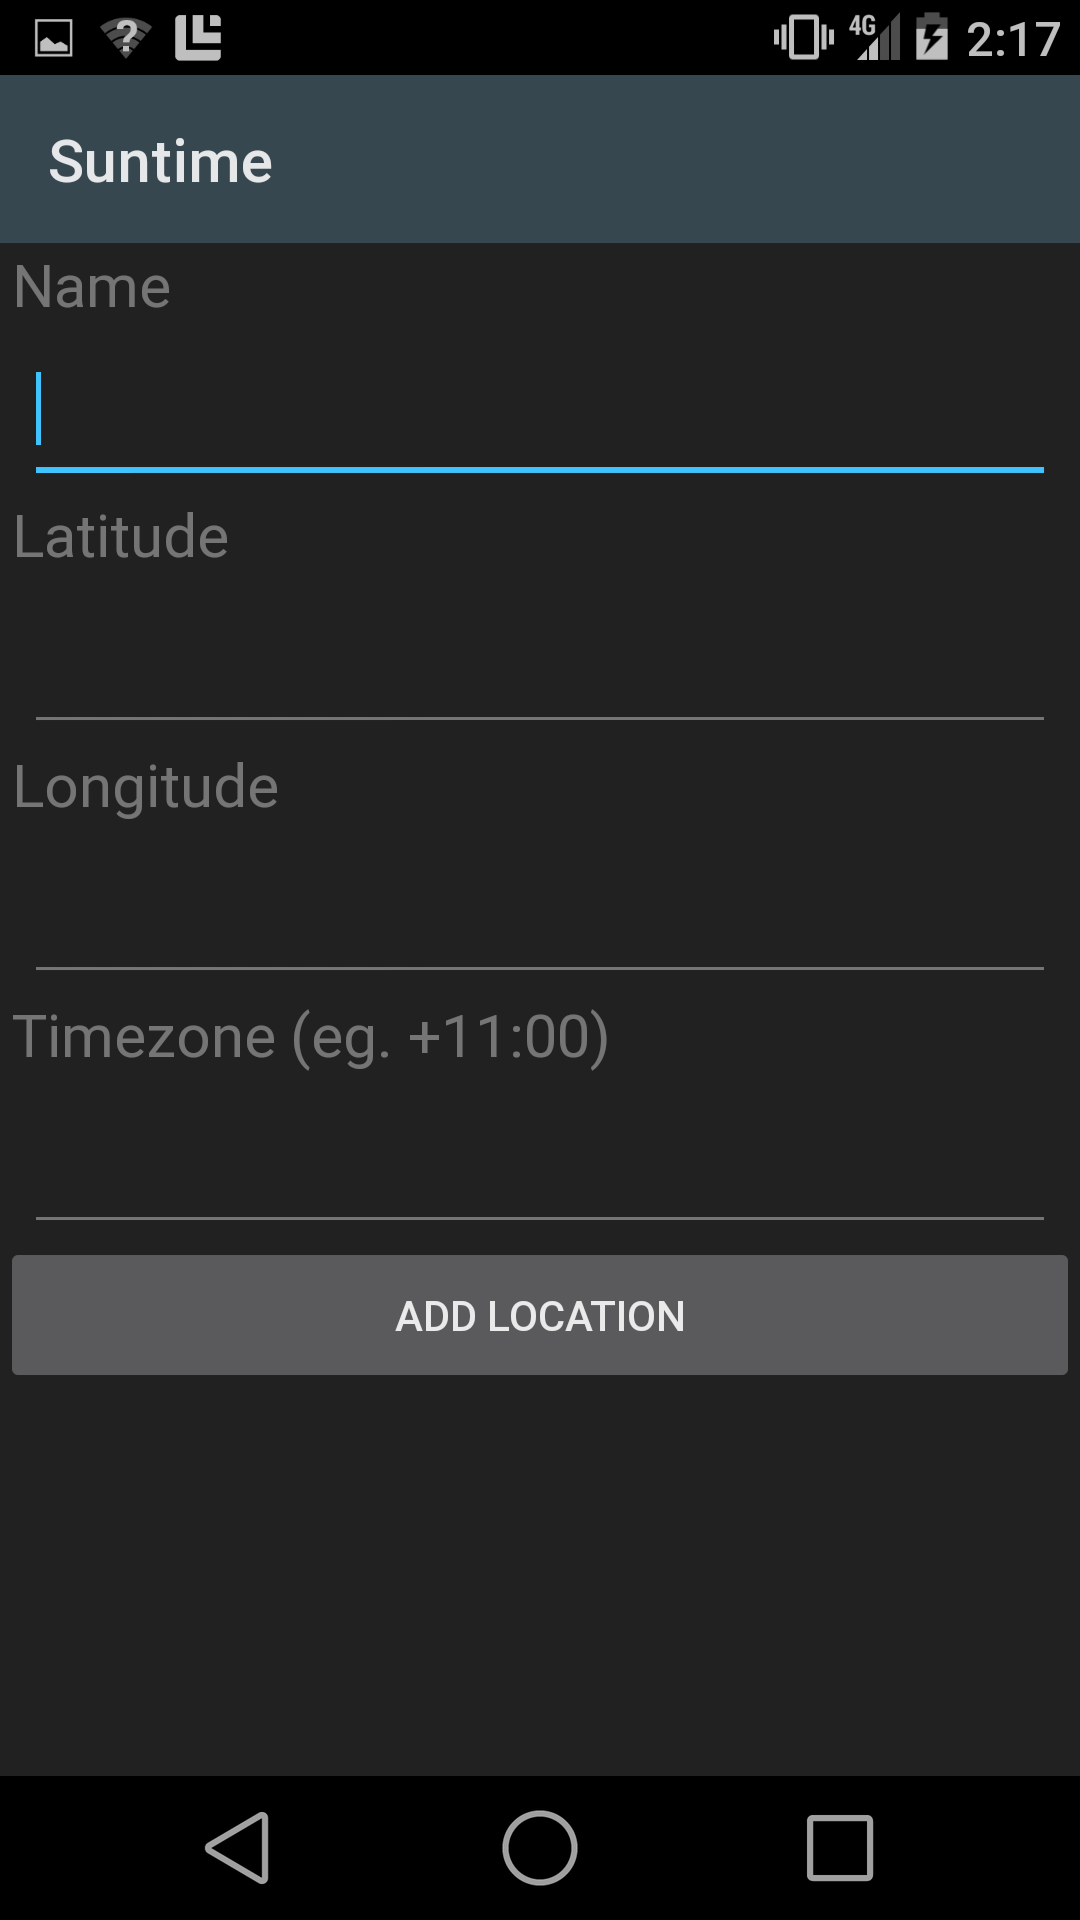
\includegraphics[width=5cm]{images/add.png}}
}\\
\end{figure}

\begin{figure}[H]
\centering{
	\fbox{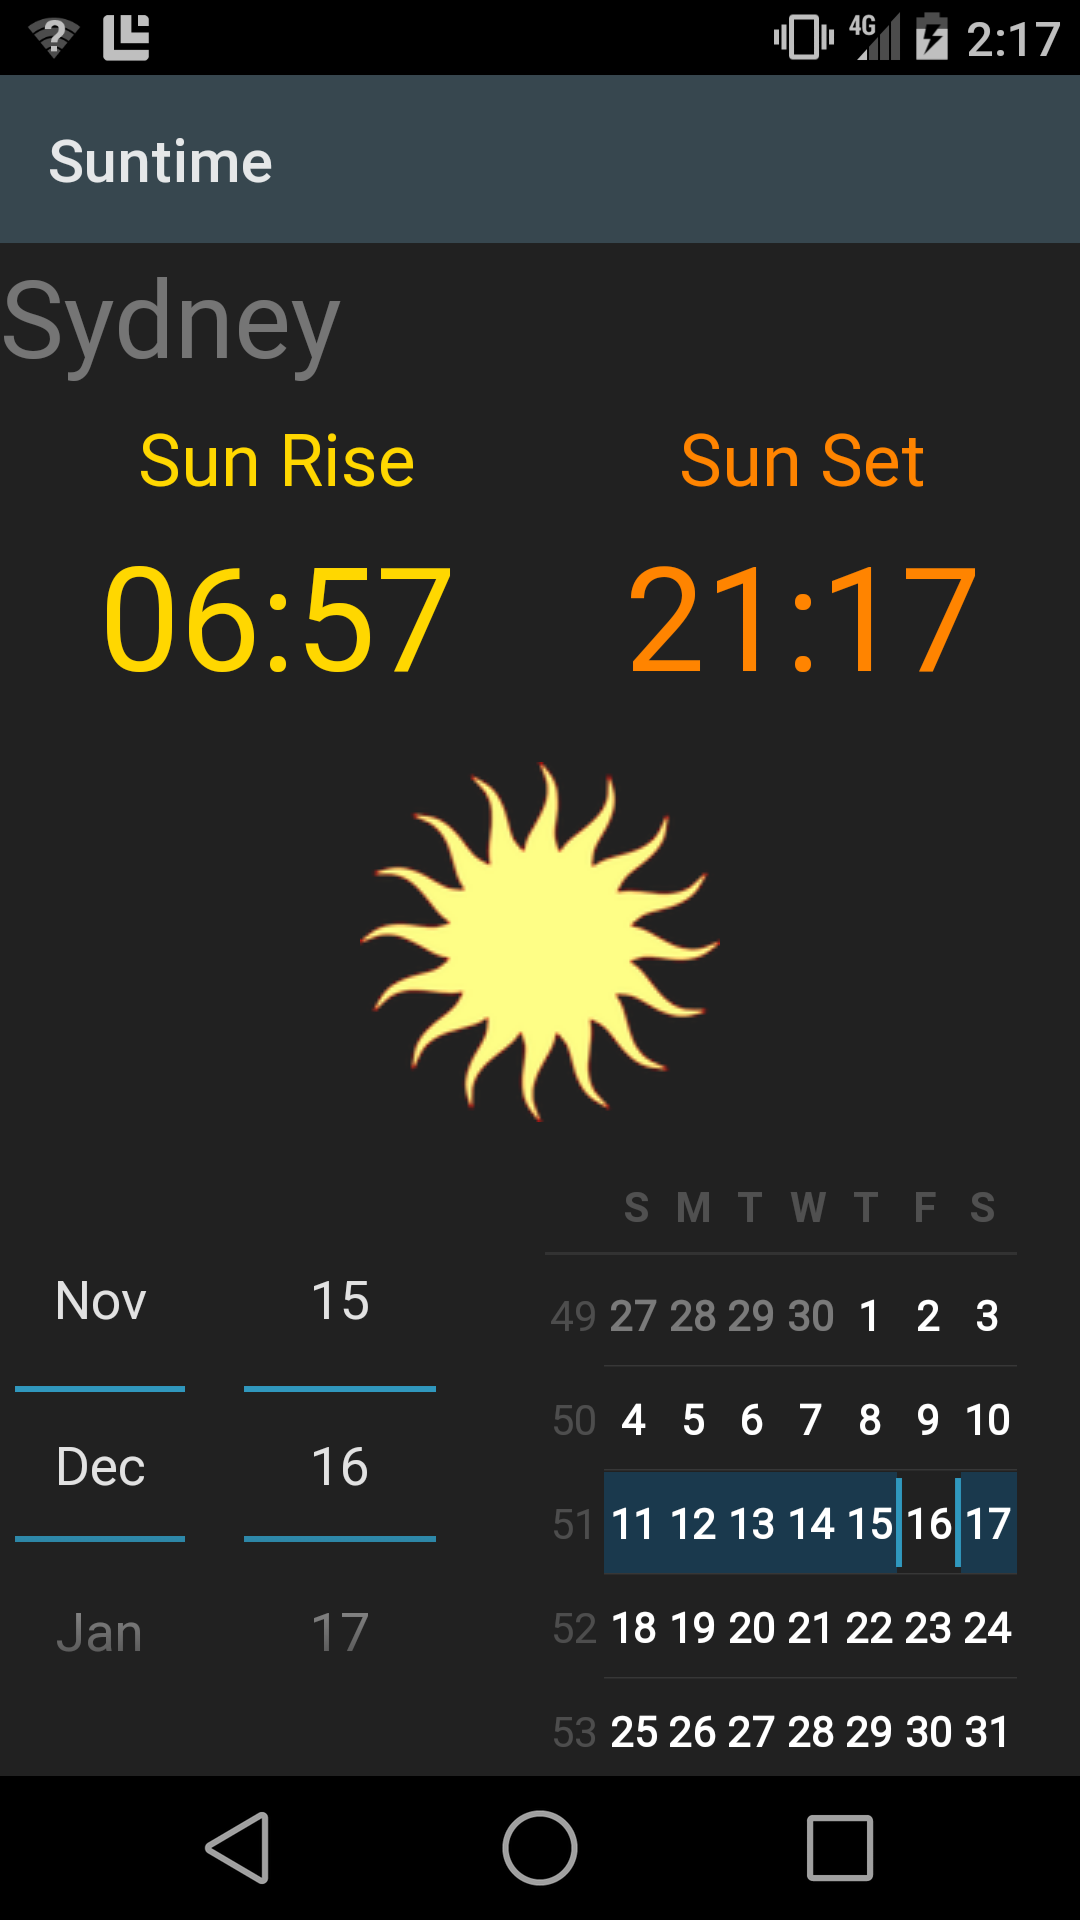
\includegraphics[width=5cm]{images/suntime.png}}
}\\
\end{figure}

\begin{landscape}
\subsection{Source Code}
\subsubsection{LocationsActivity}
\inputminted{java}{../../Apps/Suntime-Custom/app/src/main/java/au/net/danielparker/suntime/ui/LocationsActivity.java}

\subsubsection{AddNewLocation}
\inputminted{java}{../../Apps/Suntime-Custom/app/src/main/java/au/net/danielparker/suntime/ui/AddNewLocation.java}

\subsubsection{LocationsAdapter}
\inputminted{java}{../../Apps/Suntime-Custom/app/src/main/java/au/net/danielparker/suntime/ui/LocationsAdapter.java}

\subsubsection{Location}
\inputminted{java}{../../Apps/Suntime-Custom/app/src/main/java/au/net/danielparker/suntime/model/Location.java}

\subsubsection{activity\_locations}
\inputminted{xml}{../../Apps/Suntime-Custom/app/src/main/res/layout/activity_locations.xml}

\subsubsection{activity\_add\_custom}
\inputminted{xml}{../../Apps/Suntime-Custom/app/src/main/res/layout/activity_add_custom.xml}

\end{landscape}

\end{document}
